\section{Methodology}
\label{sec:methodology}

\subsection{Framework Overview}
\label{sec:method:overview}
The proposed framework addresses knowledge graph (KG) quality enhancement through a closed-loop architecture comprising two integrated components: a \textbf{multi-scale quality assessment system} and a \textbf{hybrid completion engine}. Rather than applying uniform repair heuristics across heterogeneous defects, the system decouples diagnostic evaluation from optimization execution. Given an initial KG, the assessment module evaluates relational dependencies across expanding contextual scopes to generate a diagnostic profile that quantifies scale-specific deficits. This profile is subsequently fed into the hybrid completion engine, which orchestrates targeted interventions via constraint-driven optimization and scale-aware routing. The system iteratively applies assessment, constraint verification, strategy activation, and repair until convergence criteria are satisfied or quality thresholds are met.

This design responds to a fundamental limitation in existing enhancement pipelines: quality assessment and repair are typically decoupled. Structural deduplication, logical validation, and semantic correction are treated as independent post-processing steps without a unified objective. This fragmentation frequently leads to optimization conflicts, where improvements in one metric inadvertently degrade another. Our framework resolves this by establishing a closed-loop workflow where diagnostic outputs directly govern repair actions, ensuring that every intervention is coherent with the current quality state.

A second limitation is the reliance on uniform repair strategies. Traditional methods apply identical operations to heterogeneous error types, failing to distinguish between local topological anomalies, multi-hop logical violations, and cross-context functional misalignments. This uniformity wastes computational resources on already-satisfied constraints while leaving critical violations unresolved. We address this by introducing scale-aware decomposition, which matches intervention granularity to the structural scope of the underlying defect, preventing cross-dimensional interference. Furthermore, existing LLM-assisted or heuristic repair processes often lack formal boundaries during optimization, leading to uncontrolled graph modifications and metric-induced over-optimization (reward hacking). Models may maximize surface-level scores without respecting structural or factual boundaries, introducing redundancy or propagating errors. Our framework mitigates this by embedding explicit constraint boundaries that establish verifiable quality lower limits, ensuring that repair trajectories remain within a reliable feasible region.

\begin{figure}[t]
	\centering
	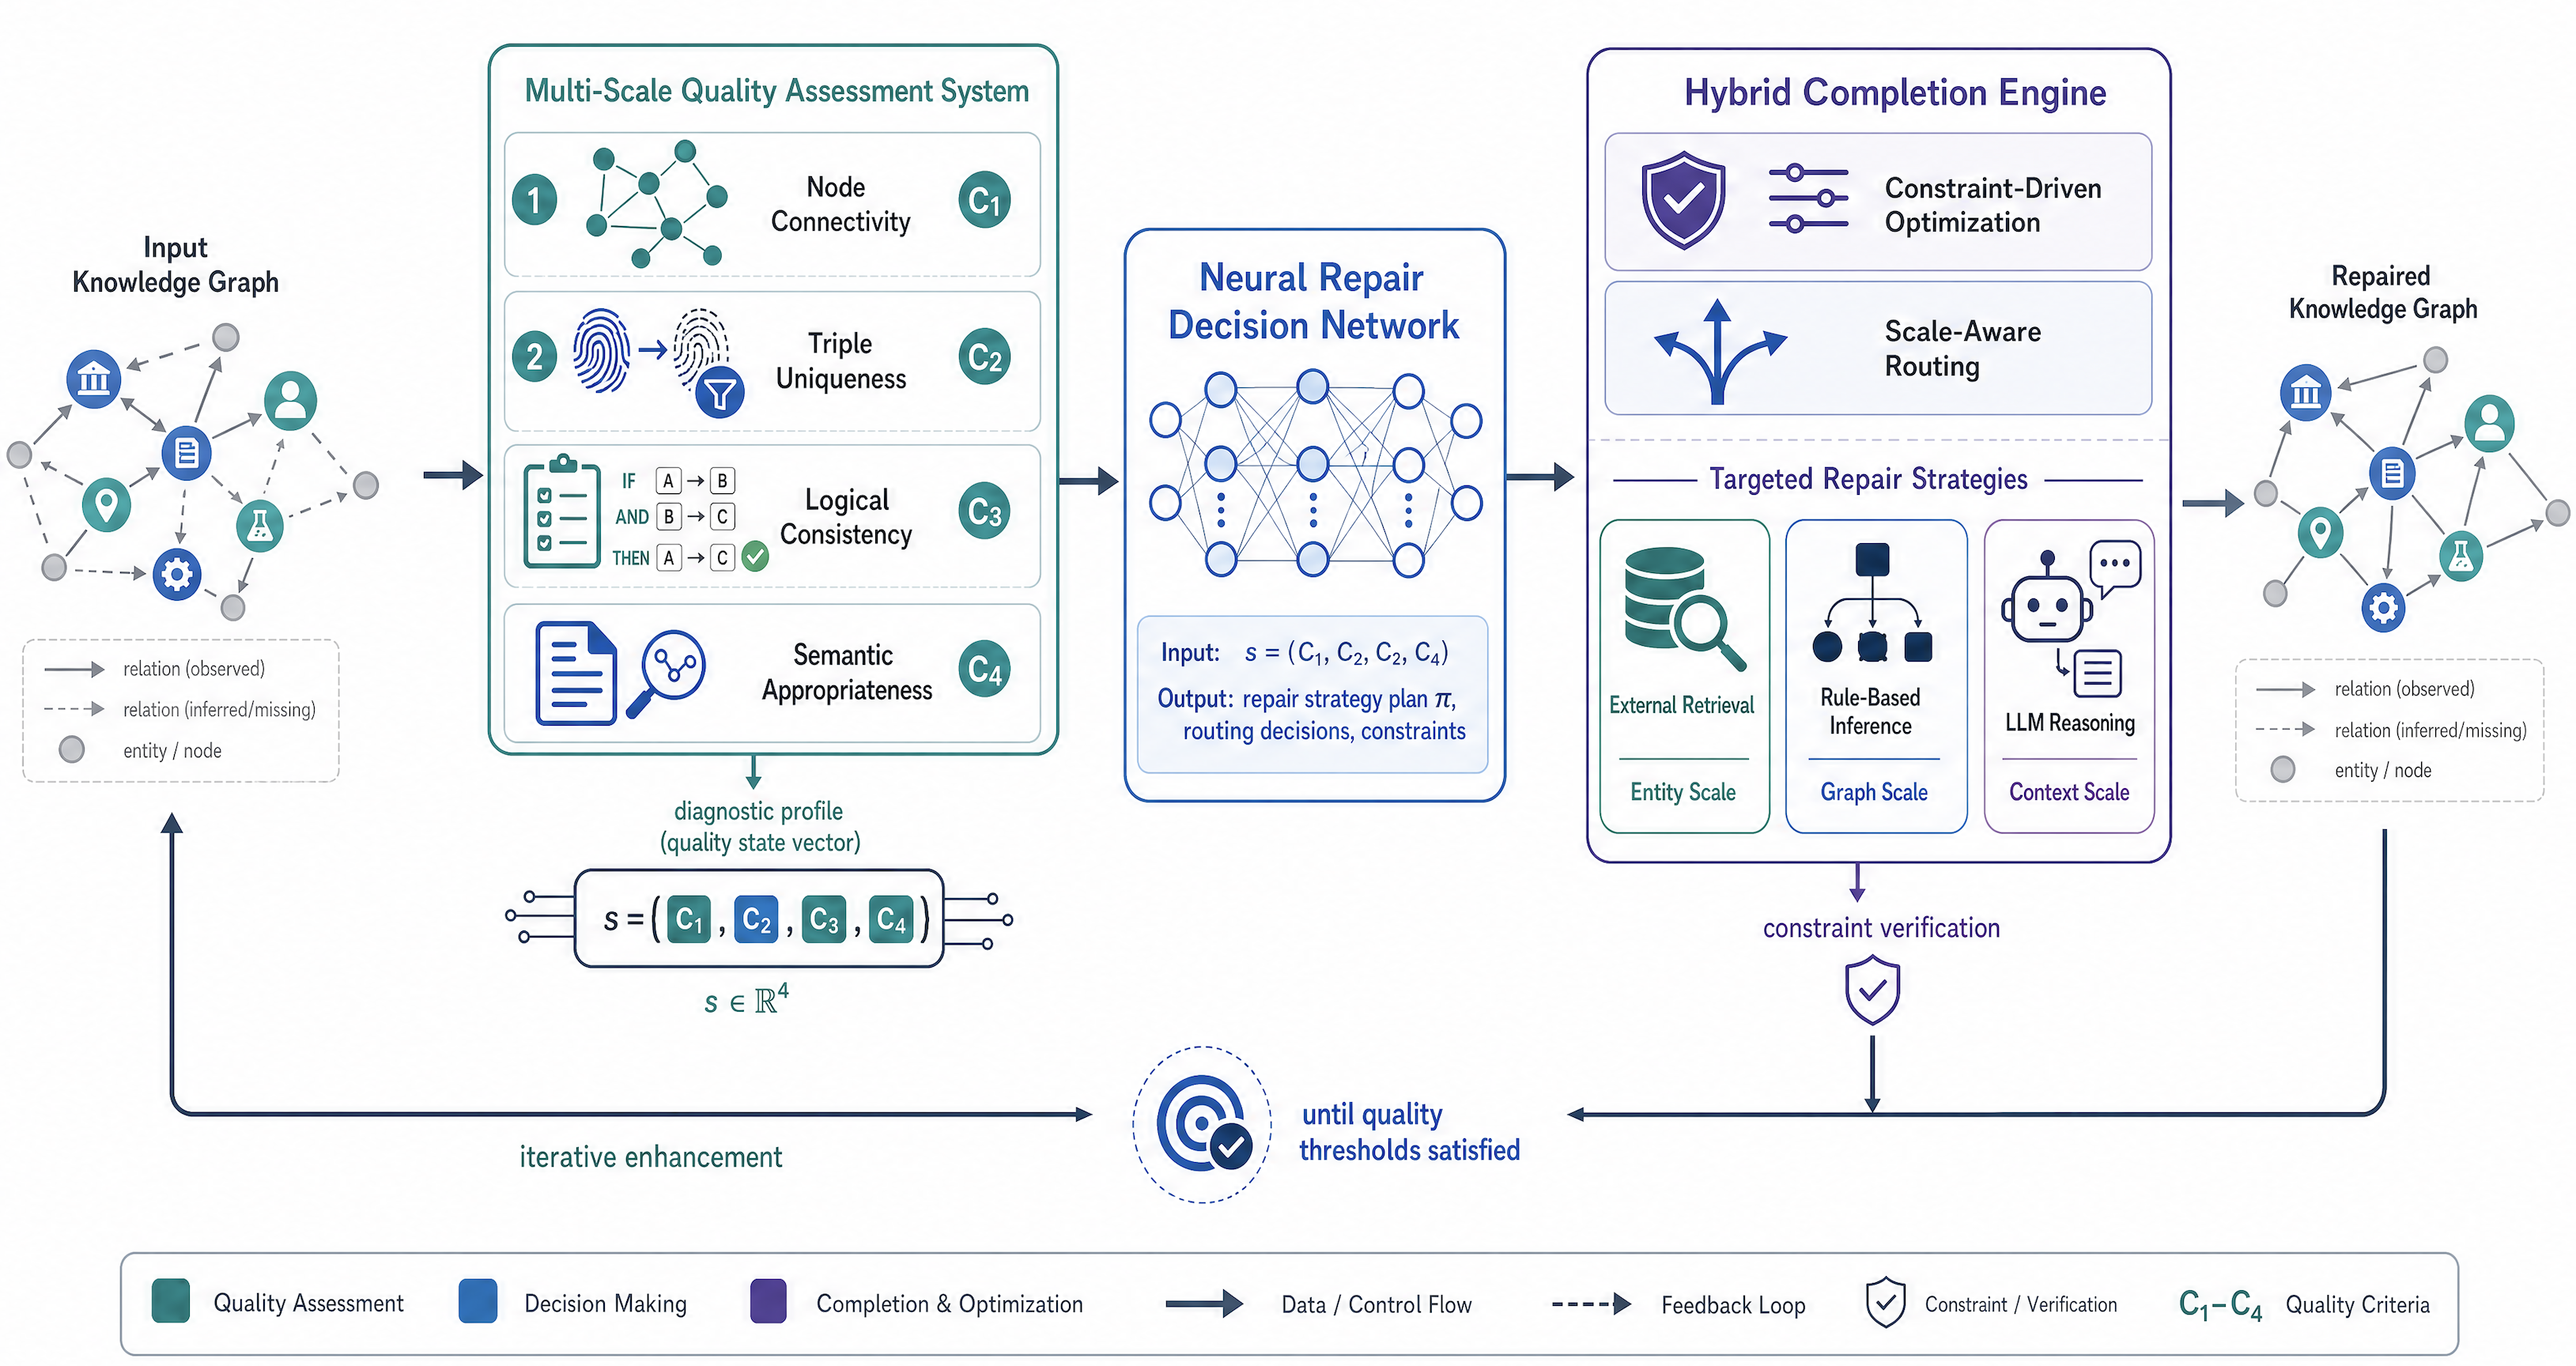
\includegraphics[width=1.0\linewidth]{figure/method/image1.png}
	\caption{Framework architecture. The multi-scale assessment system generates a diagnostic profile across entity, graph, and context scopes. The hybrid completion engine applies constraint-driven optimization and scale-aware routing to activate targeted repair strategies, iterating until quality thresholds are satisfied. }
	\label{fig:framework_overview}
\end{figure}

\subsection{Multi-Scale Quality Assessment}
\label{sec:method:assessment}
KG defects fundamentally manifest as violations of relational dependencies across increasing contextual scopes. A single validation granularity cannot capture this spectrum, as local connectivity errors, global schema contradictions, and cross-document process misalignments require distinct verification mechanisms. We therefore design a multi-scale diagnostic framework that progressively examines dependency validity, ensuring that defect localization matches the structural horizon of the underlying violation. This design is grounded in the observation that relational dependencies in knowledge representations naturally expand from explicit local connections to implicit logical structures, and finally to long-range functional and causal alignments. 

The core of our quality assessment system revolves around a unified scoring criterion that quantifies the comprehensive quality of a given graph state. We define four fundamental quality dimensions: node connectivity ($C_1$), triple uniqueness ($C_2$), logical consistency ($C_3$), and semantic appropriateness ($C_4$). Let $G'$ denote a candidate graph state reachable from the current graph by a bounded sequence of repair actions. The constrained quality criterion is formulated as:
\begin{equation}
	\label{eq:constrained_opt}
	\begin{aligned}
		\max_{G'} \quad & Q(G') = \sum_{i=1}^{4} w_i S(C_i \mid G') \\
		\text{s.t.} \quad &
		\left\{
		\begin{alignedat}{2}
			\bar{S}(C_3 \mid G') &\geq \theta_{\text{consistency}} &&\quad \text{(positive hard constraint)} \\
			\theta_{\min}^{\text{conn}} &\leq \bar{S}(C_1 \mid G') \leq \theta_{\max}^{\text{conn}} &&\quad \text{(connectivity balance)} \\
			\theta_{\min}^{\text{dens}} &\leq D(G') \leq \theta_{\max}^{\text{dens}} &&\quad \text{(density constraint)} \\
			\text{Relevance}(G') &\geq \theta_{\text{task}} &&\quad \text{(task-alignment constraint)} \\
			\bar{S}(C_2 \mid G') &\geq \theta_{\text{uniqueness}},\; \bar{S}(C_4 \mid G') \geq \theta_{\text{semantic}} &&\quad \text{(optional constraints)}
		\end{alignedat}
		\right.
	\end{aligned}
\end{equation}
where $w_i$ represents the importance weight of each quality dimension, $S(C_i \mid G') \in [0,100]$ denotes the reported scale-specific score, and $\bar{S}(C_i \mid G')=S(C_i \mid G')/100$ is the normalized score used in threshold checks. Since KGs may contain directed and multi-relational triples, the density term is computed on the undirected simple projection $E_{\mathrm{prj}}(G')=\{\{u,v\}\mid (u,r,v)\in E' \lor (v,r,u)\in E'\}$ as $D(G')=2|E_{\mathrm{prj}}(G')|/(|V'|(|V'|-1))$. Positive constraints (e.g., $\bar{S}(C_3) \geq \theta_{\text{consistency}}$) define minimum reliability thresholds, while negative constraints (e.g., density upper bounds and connectivity ceilings) prevent artificial score inflation through redundant edge addition or over-clustering. These constraints define the feasible region for repair actions and enforce checked quality boundaries; they do not by themselves prove that a feasible globally optimal graph exists or that every hard violation is repairable.

To bridge the gap between quality diagnosis and down-stream neural execution, the assessment module condenses these dimensional evaluations into a fixed-length \textbf{quality state vector}:
\begin{equation}
\label{eq:quality_state}
\mathbf{s} = \big(S(C_1), S(C_2), S(C_3), S(C_4)\big) \in [0,100]^4,
\end{equation}
which precisely localizes deficits without redundancy. This vector acts as a unified numerical interface that maps the continuous multi-scale relational dependency expansion into the downstream decision networks.

\begin{figure}[t]
	\centering
	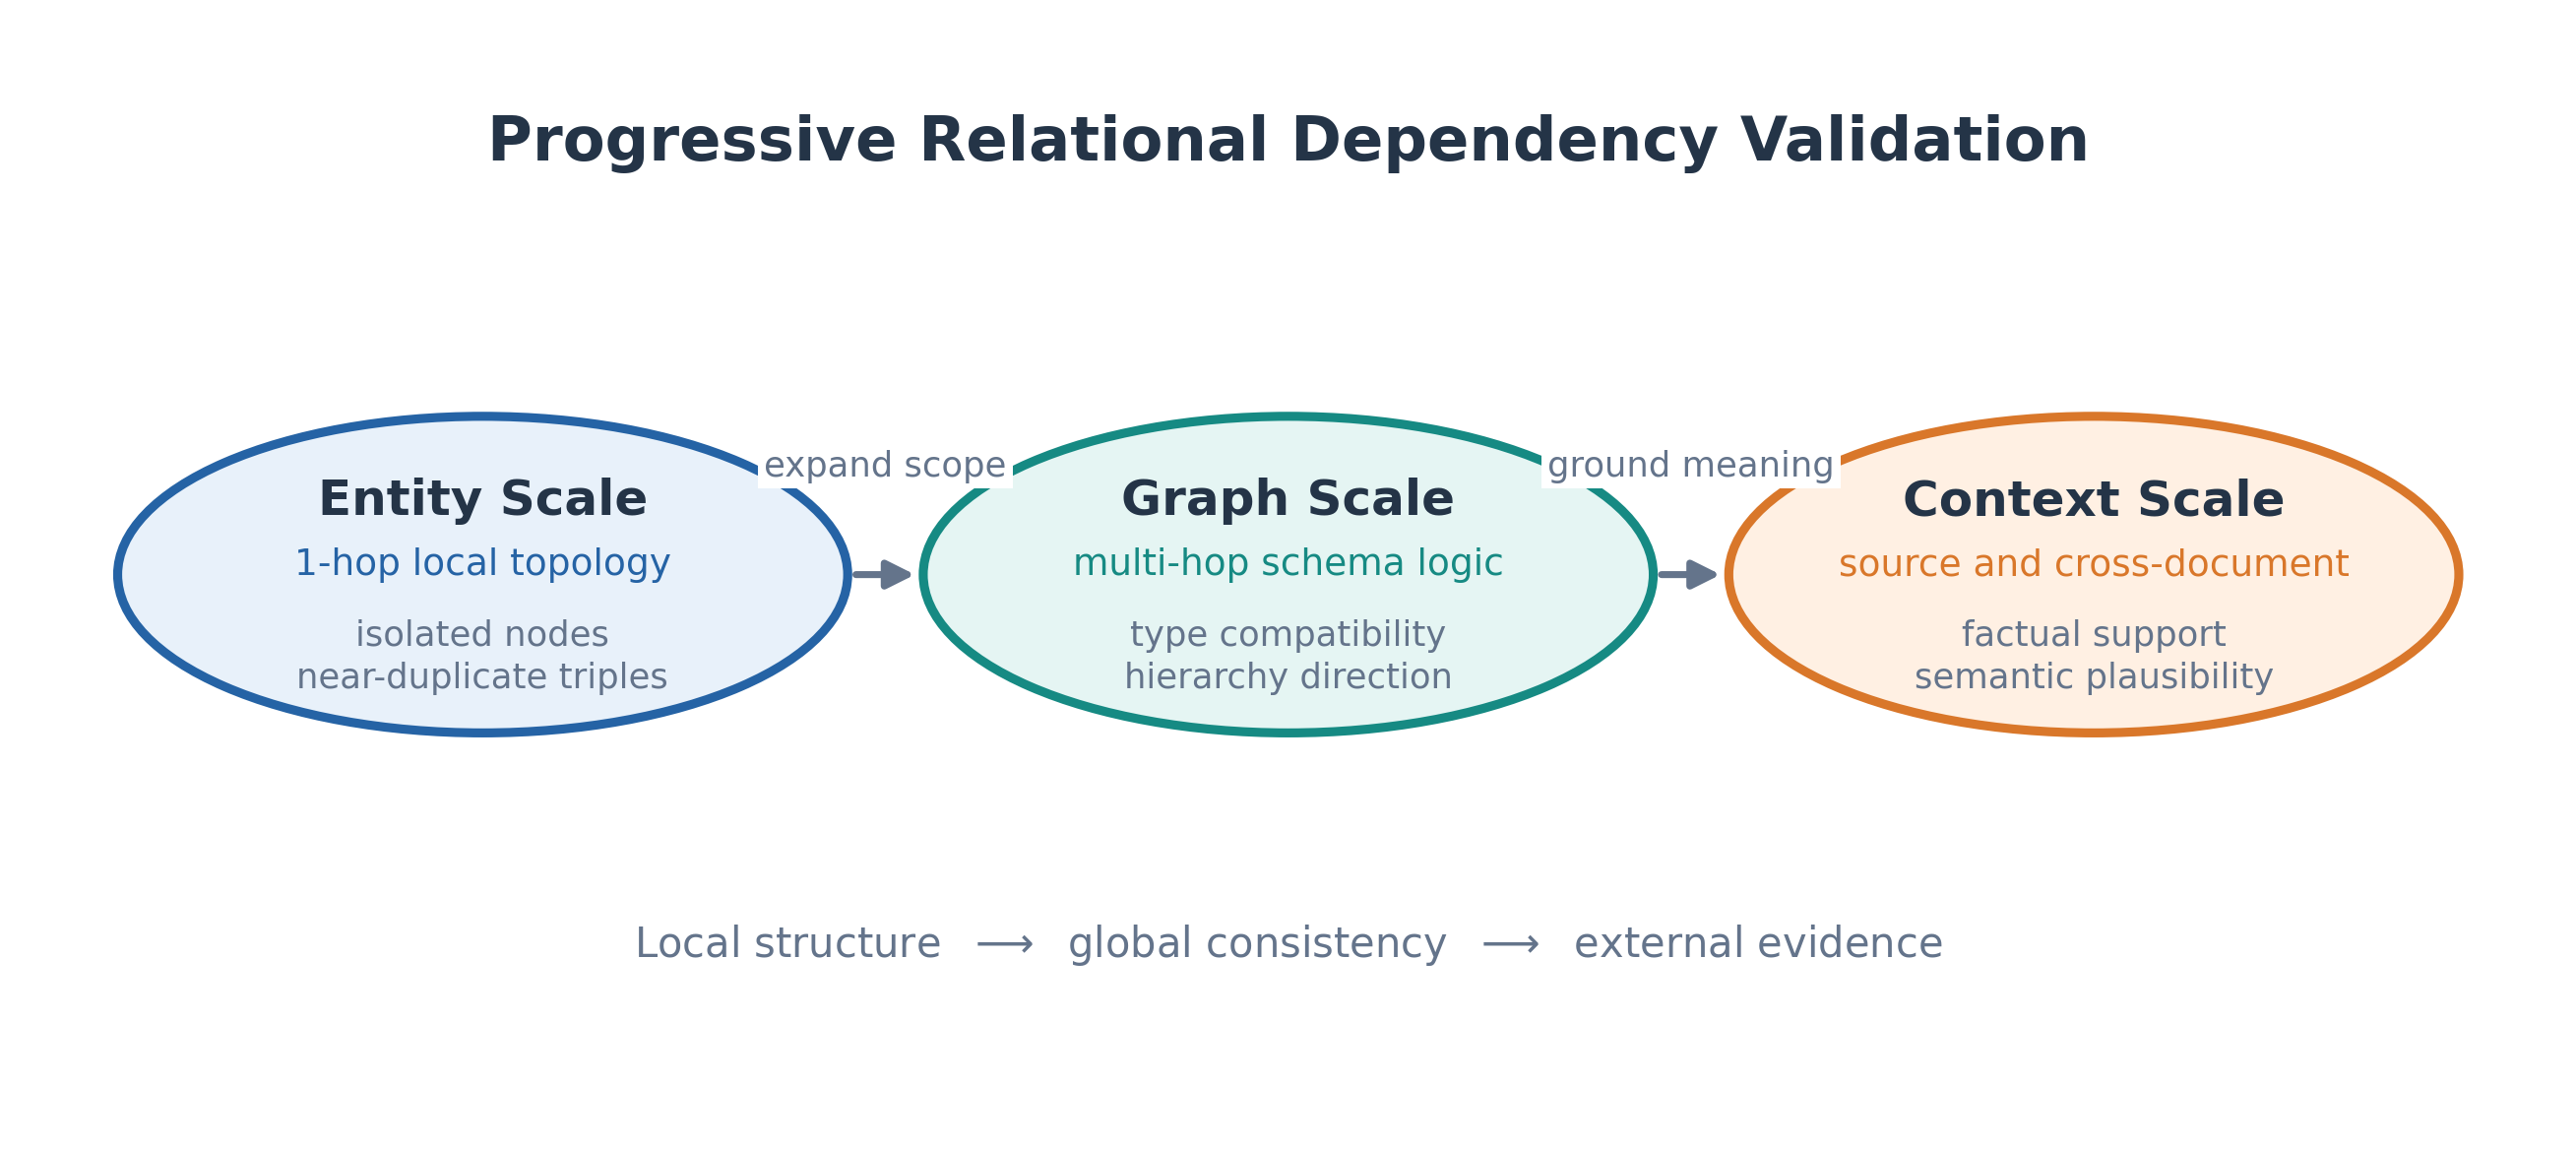
\includegraphics[width=1.0\linewidth]{figure/method/image2.png}
	\caption{Multi-scale relational dependency expansion. Validation scope progresses from local explicit connections (entity-scale) to multi-hop logical constraints (graph-scale) and finally to cross-context functional/causal alignments (context-scale).}
	\label{fig:scale_relationship}
\end{figure}

The calculation of the quality dimensions flows progressively from explicit local topologies to global, long-range contextual bounds. For node connectivity ($C_1$) and triple uniqueness ($C_2$), the system operates at the micro-topological level to capture defects violating explicit, local dependencies. Isolated entities are identified via $\deg(e)=0$, while missing relations are inferred through source text co-occurrence analysis and syntactic dependency parsing. Let $r_{\text{iso}}$ denote the isolated-node rate. We report $S(C_1)=100(1-r_{\text{iso}})$. Redundancy is quantified using weighted embedding similarity: $\text{Sim}(t_1, t_2) = \alpha \cos(\mathbf{e}_{s_1}, \mathbf{e}_{s_2}) + \beta \cos(\mathbf{e}_{r_1}, \mathbf{e}_{r_2}) + \gamma \cos(\mathbf{e}_{o_1}, \mathbf{e}_{o_2})$, where $\alpha+\beta+\gamma=1$ and $\text{Sim} > \tau_{\text{dup}}$ marks a triple pair as redundant. Given redundant-triple rate $r_{\text{red}}$, we report $S(C_2)=100(1-r_{\text{red}})$.

Moving upward, logical consistency ($C_3$) addresses defects violating implicit, multi-hop dependencies and schema compliance, utilizing constraint satisfaction engines and statistical anomaly detection. Hierarchical relations are verified for transitivity and acyclicity to ensure taxonomic subgraphs form directed acyclic graphs (DAGs), while structural anomalies are flagged using degree-based Z-score analysis ($|z(e)| > 3$). Concretely, the graph-scale checker applies three rule families per domain, analogous in spirit to SHACL/ShEx shape constraints~\cite{ref_shacl2017,ref_shex2014} and OWL domain/range reasoning~\cite{ref_sirin2007}: (i) \emph{type-compatibility} rules over \texttt{(subject-type, relation, object-type)} triples (e.g., \textit{(government agency, subordinate-to, government agency)} is permitted, whereas \textit{(lower-level unit, manages, higher-level unit)} is prohibited); (ii) \emph{hierarchy} rules that flag administrative or geographic level reversals (e.g., a district-level agency placed above its municipal counterpart); and (iii) \emph{relation-validity} rules that reject empty or undefined relation types. The current rule base comprises $25/29/34$ type-compatibility rules for the government/finance/environment domains (of which $8/10/10$ are explicit prohibitions), plus the hierarchy and relation-validity checks; the complete rule set is released with our code. Given logical-conflict rate $r_{\text{log}}$, we report:
\begin{equation}
\label{eq:score_c3}
S(C_3)=100\bigl(1-r_{\text{log}}\bigr).
\end{equation}
Finally, semantic appropriateness ($C_4$) evaluates cross-boundary functional dependencies and real-world operational plausibility. It combines path-reachability verification with low-temperature LLM sampling aggregated over $K$ triples to bound variance, checking causal temporal ordering and step preconditions. If the sampled triples receive evaluator scores $s_k\in[0,1]$, we report $S(C_4)=100K^{-1}\sum_{k=1}^{K}s_k$. This multi-layered computational scheme outputs the complete profile $\mathbf{s}$, establishing a robust, multi-dimensional trustworthiness baseline.

\subsection{Neural Repair Decision Network}
\label{sec:method:decision}
Between assessment and execution, the framework introduces an explicit decision stage that determines whether enhancement should be triggered. Specifically, a lightweight neural network $f_{\phi}$ maps the quality state vector $\mathbf{s}$ (and optional auxiliary graph statistics $\mathbf{g}$ such as $|V|,|E|$, density, and violation counts) to (i) a repair decision and (ii) a scale-prior vector:
\begin{equation}
\label{eq:decision_net}
\big(p_{\text{repair}},\; \boldsymbol{\pi}\big) = f_{\phi}([\mathbf{s};\mathbf{g}]), \quad p_{\text{repair}}\in[0,1],\; \boldsymbol{\pi}\in\Delta^2.
\end{equation}
Here $\Delta^2=\{\boldsymbol{\pi}\in\mathbb{R}_{\geq 0}^3:\sum_j \pi_j=1\}$ denotes the three-class probability simplex. At inference time, the system executes enhancement only if $p_{\text{repair}} \ge \tau_{\text{repair}}$. When triggered, $\boldsymbol{\pi}=(\pi_{\text{entity}},\pi_{\text{graph}},\pi_{\text{context}})$ provides a soft prior over structural scopes and is passed to the routing module to bias strategy activation.

\paragraph{Self-supervised training signals.} To avoid expensive human annotations, we train $f_{\phi}$ using supervision automatically derived from the constraint checker and diagnostic outputs. Let $\mathcal{V}(G)$ denote the detected violation set and $\mathcal{V}_{\text{hard}}(G)\subseteq\mathcal{V}(G)$ denote the hard-constraint violations. We define a binary repair label
\begin{equation}
\label{eq:repair_label}
 y = \mathbf{1}\big[\mathcal{V}_{\text{hard}}(G)\neq\emptyset\;\lor\; Q(G) < \theta_{Q}\big],
\end{equation}
where $\theta_{Q}$ is a target comprehensive quality threshold. In addition, we derive a scale attribution label $\mathbf{y}_{\text{scale}}\in\Delta^2$ by counting violations per originating scope:
\begin{equation}
\label{eq:scale_label}
\mathbf{y}_{\text{scale}} = \mathrm{Normalize}\big(|\mathcal{V}_{\text{entity}}|,\;|\mathcal{V}_{\text{graph}}|,\;|\mathcal{V}_{\text{context}}|\big).
\end{equation}
Here $\mathrm{Normalize}(\mathbf{c})=\mathbf{c}/\sum_j c_j$ when $\sum_j c_j>0$; clean instances with no detected violation are used for the binary repair head but are masked out of the scale-prior loss. The decision network is trained by minimizing a joint objective
\begin{equation}
\label{eq:decision_loss}
\mathcal{L}(\phi)=\mathrm{BCE}(p_{\text{repair}},y)+\lambda\,m_{\text{scale}}\,\mathrm{CE}(\mathbf{y}_{\text{scale}},\boldsymbol{\pi}).
\end{equation}
where $m_{\text{scale}}=\mathbf{1}[\sum_j c_j>0]$, $\mathrm{BCE}$ is binary cross-entropy, and $\mathrm{CE}$ is multiclass cross-entropy over the three scale classes.

The learned prior $\boldsymbol{\pi}$ is subsequently incorporated into the routing mechanism as a soft bias rather than a hard gate to preserve search flexibility. For a detected violation $v$ attributed to scale $\sigma(v)$ and a candidate action $a\in\mathcal{A}_{\text{cand}}(v)$ with base utility $u(a\mid v)$ derived from deficit severity and estimated edit cost, we define the biased utility:
\begin{equation}
\label{eq:routing_bias}
\tilde{u}(a\mid v)=u(a\mid v)+\eta\log\big(\pi_{\sigma(v)}+\epsilon_{\log}\big),
\end{equation}
where $\eta$ controls the strength of the neural prior and $\epsilon_{\log}$ is a small constant to avoid numerical issues when $\pi_{\sigma(v)}$ is close to zero. Structurally, the base utility is explicitly formulated as $u(a \mid v) = \widehat{\Delta Q}(a \mid v) - \beta\,\mathrm{cost}(a)$, which balances localized comprehensive quality gains against the operational destructiveness of the intervention modality. This design improves efficiency by prioritizing the most likely defect scope while preserving constraint-driven feasibility checks in the optimization stage.

\subsection{Hybrid Completion Engine}
\label{sec:method:engine}
The hybrid completion engine serves as the decision-making core that transforms diagnostic profiles into targeted graph modifications. Rather than executing blind repair operations, the engine operates under two synergistic mechanisms: constraint-driven optimization defines the feasible region and directional gradients for enhancement, while scale-aware routing dynamically allocates repair strategies according to diagnosed deficit patterns. These mechanisms are coupled with a suite of targeted repair modalities—external retrieval, LLM reasoning, and rule-based inference—that provide the actual intervention primitives. By decoupling boundary definition, strategy routing, and execution tools, the engine ensures that every repair action is precisely scoped, computationally efficient, and minimally destructive.

The scale-aware routing module acts as the precision filter that maps diagnostic outputs to strategy activation signals. Given the diagnostic profile $\mathbf{s}$ and detected violation set $\mathcal{V}$, the routing function $\mathcal{R}(\mathbf{s}, \mathcal{V})$ identifies the originating scope for each violation and selects a subset of candidate repair actions from the available modalities. For entity-scale violations (e.g., isolated nodes or low redundancy scores), the router prioritizes external retrieval and syntactic co-occurrence analysis to recover missing connections without altering established logical patterns. For graph-scale violations (e.g., hierarchical conflicts or constraint breaches), the router activates rule-based engines and LLM reasoning to propagate constraints and resolve domain/range mismatches. For context-scale violations (e.g., causal gaps or semantic inaccuracies), the router triggers process simulation checks and counterfactual LLM prompts to validate long-range dependencies. This mapping yields cross-scale isolation, adaptive resource allocation, and computational throttling.

The repair modalities constitute the execution layer of the hybrid completion engine, providing concrete intervention primitives optimized for specific scale contexts and constraint types. External Retrieval queries authoritative knowledge sources to recover missing attributes; LLM Reasoning leverages contextual inference to deduce implicit relations; Rule-Based Inference applies domain-specific logical templates for deterministic completion. To prevent aggressive pruning that could fragment valid subgraphs, all modalities operate under a least-destructive cost hierarchy:
\begin{equation}
	\text{cost}(a) = \begin{cases}
		\lambda_{\text{del}} & \text{if } a = \text{delete} \\
		\lambda_{\text{ret}} & \text{if } a = \text{retype} \\
		\lambda_{\text{cmp}} & \text{if } a = \text{complete}
	\end{cases}, \quad \text{where } \lambda_{\text{del}} > \lambda_{\text{ret}} > \lambda_{\text{cmp}}.
\end{equation}
This cost structure functions as a negative constraint implementation, explicitly penalizing the removal of high-confidence information and favoring completion or re-typing over deletion, ensuring that every repair action adheres to the principle of minimal intervention.

\subsection{Iterative Enhancement Algorithm}
\label{sec:method:algorithm}
The iterative enhancement algorithm unifies the assessment system, completion engine, and constraint logic into a closed-loop optimization procedure. Rather than executing a single-pass repair, the algorithm repeatedly cycles through diagnostic evaluation, constraint verification, strategy routing, and utility-maximizing modification until convergence criteria are satisfied. This iterative design allows the system to dynamically adjust its intervention strategy as the graph topology evolves, preventing early repair actions from inadvertently triggering secondary violations in subsequent scales.

\begin{figure}[t]
	\centering
	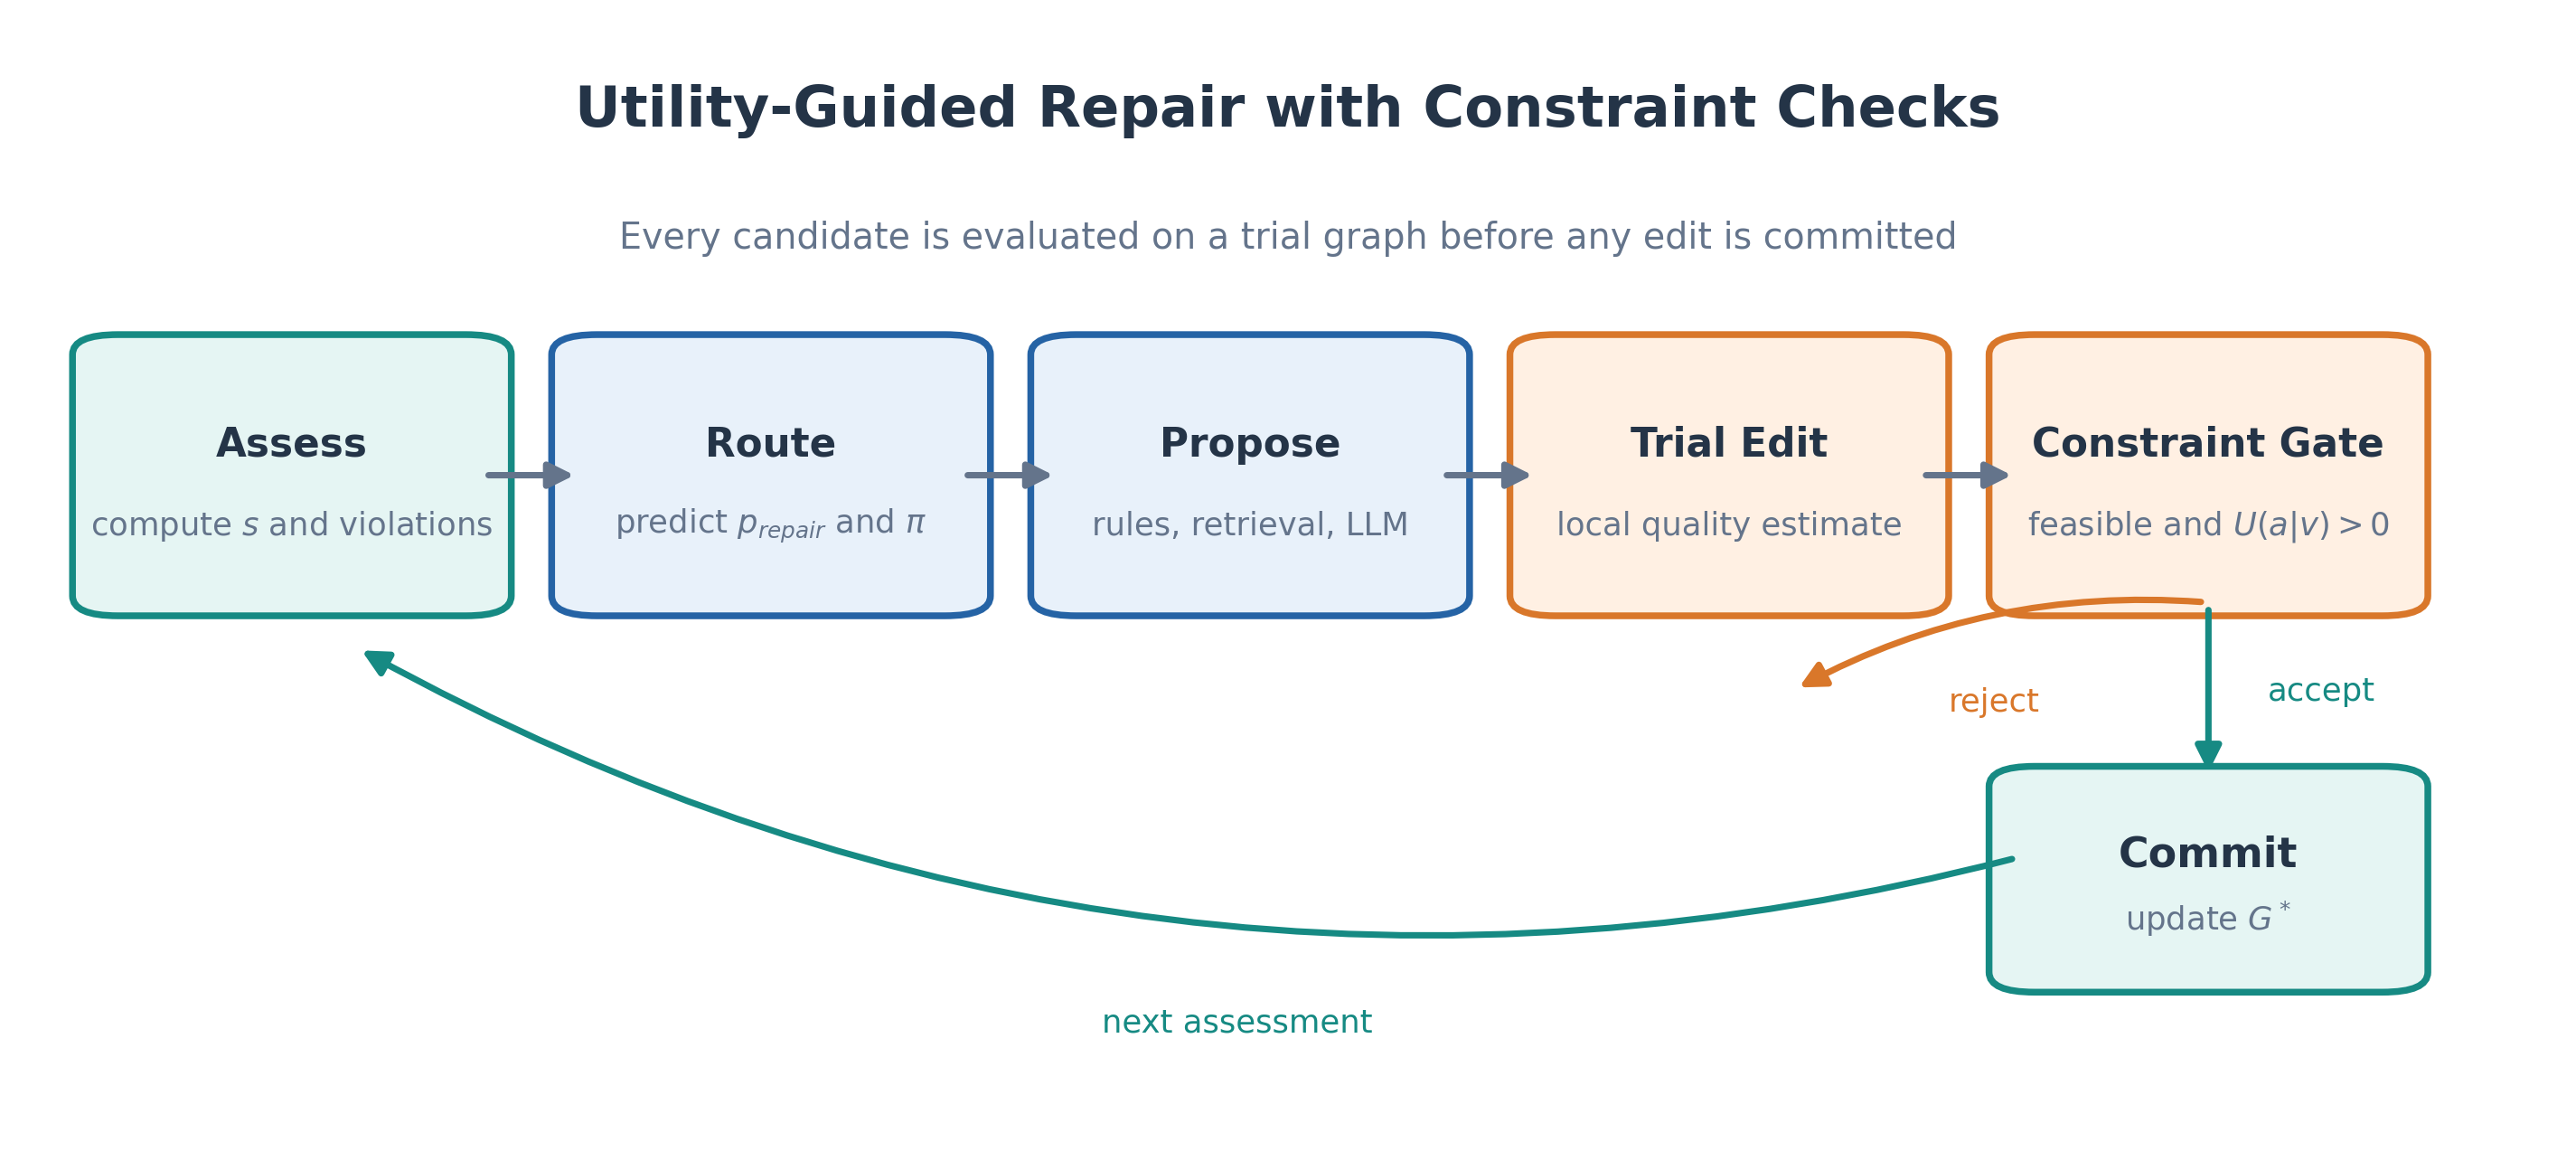
\includegraphics[width=1.0\linewidth]{figure/method/image3.png}
	\caption{Optimization and routing flow. The multi-strategy collaborative analysis framework processes scale-specific diagnostics through a synthesis engine, generating targeted defect repair plans that feed into the enhanced KG. Continuous iteration ensures convergence within constraint boundaries.}
	\label{fig:optimization_flow}
\end{figure}

Algorithm~\ref{alg:enhancement} formalizes the enhancement procedure. At each iteration, the system computes the multi-scale quality vector $\mathbf{s}$ and identifies constraint violations $\mathcal{V}$. The scale-aware router maps violations to candidate actions, and the optimizer selects an action $a^*$ that maximizes an explicit objective. For a violation $v$ and candidate actions $\mathcal{A}_{\text{cand}}(v)$, we define the neural-biased optimization utility as:
\begin{equation}
\label{eq:action_utility}
U(a\mid v)=\widehat{\Delta Q}(a\mid v)-\beta\,\mathrm{cost}(a) + \eta\log\big(\pi_{\sigma(v)}+\epsilon_{\log}\big),
\end{equation}
where $\beta$ trades off quality improvement against intervention destructiveness, $\epsilon_{\log}$ ensures numerical stability, and $\eta\log\big(\pi_{\sigma(v)}+\epsilon_{\log}\big)$ integrates the soft guidance from the decision network. To keep computation tractable on large-scale KGs and avoid full-graph rescoring for every candidate action, the estimated comprehensive quality gain $\widehat{\Delta Q}(a \mid v)$ is computed via a localized closed-form check over the $k$-hop neighborhood of the affected entities: $\widehat{\Delta Q}(a \mid v) = \sum_{i=1}^4 w_i [ S(C_i \mid G^* \oplus a) - S(C_i \mid G^*) ]_{k\text{-hop}}$.

The global comprehensive quality score $Q(G)$ is iteratively updated, and convergence is declared when the per-iteration gain falls below $\epsilon_{\text{conv}}$. An action $a^*$ is committed only if it has positive utility and does not breach the keep-out boundaries of Eq.~(\ref{eq:constrained_opt}). Because $\widehat{\Delta Q}$ is a localized $k$-hop approximation, we do not claim formal global monotonicity: in principle, a committed edit could perturb long-range dependencies outside its $k$-hop window and lower the global score. In practice the trajectory is well behaved---the feasibility checks prevent constraint-violating commits, and the comprehensive score rose monotonically and converged within a few iterations in all our runs (Section~\ref{sec:eval:sensitivity}). When stricter guarantees are needed, a periodic global re-evaluation with rollback of any non-improving step can be enabled as a safeguard at additional cost; quantifying the local-approximation error is left to future work.

\begin{algorithm}[H]
	\caption{Constraint-Driven Multi-Scale KG Enhancement}
	\label{alg:enhancement}
	\begin{algorithmic}[1]
		\Require Knowledge graph $G$, constraint set $\mathcal{C}$, weights $\mathbf{w}$, thresholds $\Theta$, max iterations $T$
		\Ensure Enhanced knowledge graph $G^*$
		\State $G^* \gets G$
		\State $\mathbf{s}^{(0)} \gets \text{MultiScaleEvaluate}(G^*)$
		\State $Q_{\text{prev}} \gets \sum_{i=1}^4 w_i S^{(0)}(C_i)$ \Comment{Initialize global quality score}
		\For{$t = 1$ \textbf{to} $T$}
		\State $\mathbf{s} \gets \text{MultiScaleEvaluate}(G^*)$ \Comment{Compute quality state vector}
		\State $\mathbf{g} \gets \text{GraphStats}(G^*)$
		\State $(p_{\text{repair}},\boldsymbol{\pi}) \gets f_{\phi}([\mathbf{s};\mathbf{g}])$
		\If{$p_{\text{repair}} < \tau_{\text{repair}}$}
			\State \textbf{break}
		\EndIf
		\State $\mathcal{V} \gets \text{DetectViolations}(\mathbf{s}, \mathcal{C})$
		\If{$\mathcal{V} == \emptyset$} \Comment{Early termination if constraints satisfied}
			\State \textbf{break}
		\EndIf
		\State $\mathcal{V} \gets \text{PrioritizeHardViolations}(\mathcal{V}, \mathcal{C})$
		\State $\mathcal{A}_{\text{cand}} \gets \mathcal{R}(\mathbf{s}, \mathcal{V})$ \Comment{Scale-aware routing with neural priors}
		\For{each violation $v \in \mathcal{V}$}
			\State $\mathcal{A}_{\text{feasible}} \gets \{a \in \mathcal{A}_{\text{cand}}(v) \mid \text{Apply}(G^*, a) \text{ satisfies Eq. (\ref{eq:constrained_opt}) and } U(a\mid v)>0\}$
			\If{$\mathcal{A}_{\text{feasible}} \neq \emptyset$}
				\State $a^* \gets \arg\max_{a \in \mathcal{A}_{\text{feasible}}} \; U(a\mid v)$ \Comment{Maximize neural-biased utility}
				\State $G^* \gets \text{Apply}(G^*, a^*)$
			\EndIf
		\EndFor
		\State $\mathbf{s}_{\text{new}} \gets \text{MultiScaleEvaluate}(G^*)$
		\State $Q_{\text{curr}} \gets \sum_{i=1}^{4} w_i\,\mathbf{s}_{\text{new},i}$ \Comment{Recompute comprehensive quality score}
		\If{$Q_{\text{curr}} - Q_{\text{prev}} < \epsilon_{\text{conv}}$} \Comment{Convergence check}
			\State \textbf{break}
		\EndIf
		\State $Q_{\text{prev}} \gets Q_{\text{curr}}$
		\EndFor
		\State \Return $G^*$
	\end{algorithmic}

\end{algorithm}

By coupling multi-scale diagnosis with constraint-bound optimization, the algorithm performs a feasible, utility-guided greedy search over candidate repairs. The feasibility checks bound each committed edit, while the localized utility and stopping rule make the procedure computationally efficient. In practice, the iterative loop converges within $T \leq 5$ iterations across all evaluated domains and exhibits monotonic score increases in our measured runs.
